% lecture10.tex — 1-Manifolds and Some Consequences

\section{1-Manifolds and Some Consequences}

\begin{theorem}{Classification of 1-Manifolds}{classification-1-manifolds}
    Every compact, connected 1-manifold with boundary is diffeomorphic to $S^1$ or $I = [0,1]$.
\end{theorem}

(See the Appendix of Milnor or Guillemin--Pollack for the proof. The idea is to parametrize the 1-manifold by arc length, in a maximal way.)

\begin{corollary}{Boundary Has Even Cardinality}{boundary-even}
    The boundary of any compact 1-manifold with boundary consists of an even number of points.
\end{corollary}

As we will see, this seemingly trivial corollary has numerous nontrivial applications.

Later, in the next chapter, we will refine this statement by counting those boundary points with sign (orientation). Such signed count is always $0$, and this fact is at the heart of \emph{oriented intersection theory}.

\subsection{No Retraction Lemma}

Let $M$ be a compact manifold with boundary.

\begin{lemma}{No Retraction}{no-retraction}
    There's no smooth map $f \colon M \to \partial M$ that leaves $\partial M$ pointwise fixed. That is, there is no retraction of $M$ onto $\partial M$.
\end{lemma}

\begin{proof}
    Suppose there were such a map $f$. Let $y \in \partial M$ be a regular value for $f$ (which exists thanks to Sard). Since $y$ is certainly a regular value for the identity map $f|_{\partial M}$ as well, $f^{-1}(y)$ is a smooth 1-manifold, with boundary
    \[
        \partial f^{-1}(y) = f^{-1}(y) \cap \partial M = \{y\}.
    \]
    But $f^{-1}(y)$ is also compact, so that $\#|\partial f^{-1}(y)|$ must be even, a contradiction.
\end{proof}

\subsection{Brouwer Fixed Point Theorem}

\begin{theorem}{Smooth Brouwer Fixed Point Theorem}{smooth-brouwer}
    Any smooth map $g \colon D^n \to D^n$ has a fixed point.
\end{theorem}

\begin{proof}
    Suppose $g$ has no fixed point. Then we can construct a retraction $f \colon D^n \to S^{n-1}$ which is impossible from the lemma:
    \begin{center}
    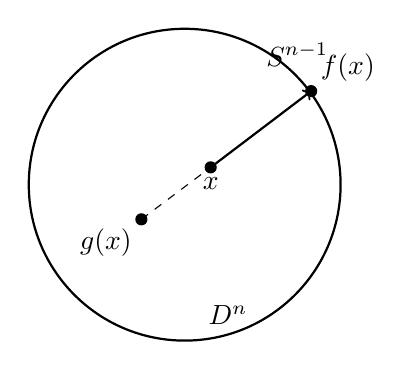
\begin{tikzpicture}[scale=1.1]
        % Disk
        \draw[thick] (0,0) circle (1.8);
        \node at (1.3,1.5) {$S^{n-1}$};
        \node at (0.5,-1.5) {$D^n$};
        % Points
        \fill (0.3,0.2) circle (2pt) node[below] {$x$};
        \fill (-0.5,-0.4) circle (2pt) node[below left] {$g(x)$};
        % Ray from g(x) through x to boundary
        \draw[dashed] (-0.5,-0.4) -- (0.3,0.2);
        \draw[->,thick] (0.3,0.2) -- (1.46,1.08);
        \fill (1.46,1.08) circle (2pt) node[above right] {$f(x)$};
    \end{tikzpicture}
    \end{center}
    \[
        f(x) = x + tu, \quad \text{where } u = \frac{x - g(x)}{\|x - g(x)\|} \text{ and } t = -x \cdot u + \sqrt{1 - x \cdot x + (x \cdot u)^2}.
    \]
    Note $t$ is strictly positive.
\end{proof}

Often, one can use an approximation theorem to pass to the continuous case, and this theorem is an example:

\begin{theorem}{Brouwer Fixed Point Theorem}{brouwer}
    Any continuous map $G \colon D^n \to D^n$ has a fixed point.
\end{theorem}

\begin{proof}
    Given $\varepsilon > 0$, thanks to the Weierstrass approximation theorem, there is a polynomial function $P_0 \colon \R^n \to \R^n$ with $\|P_0(x) - G(x)\| < \varepsilon$ for $x \in D^n$.

    However, $P_0$ may send points of $D^n$ into points outside of $D^n$, so to correct this we set $P(x) = \frac{P_0(x)}{1 + \varepsilon}$.

    Clearly, $P \colon D^n \to D^n$ and $\|P(x) - G(x)\| < \frac{2\varepsilon}{1+\varepsilon} < 2\varepsilon$ for $x \in D^n$.

    Suppose $G$ has no fixed points. Then the continuous function $\|G(x) - x\|$ must take on a minimum $\mu > 0$ on $D^n$. Choosing $P \colon D^n \to D^n$ as above, with $\|P(x) - G(x)\| < \mu$ for all $x \in D^n$, we have $P(x) \neq x$ for all $x \in D^n$.

    Since $P$ is smooth, this contradicts the Smooth Brouwer fixed point theorem.
\end{proof}

\subsection{The Hex Theorem}

The following is just for fun:

\begin{theorem}{Hex Theorem}{hex}
    There's no draw in the game of Hex. That is, if we color the vertices of a triangulation of $I^2$ in 2 colors, say red and blue, then either the red connects E--W or the blue connects N--S.
\end{theorem}

\begin{proof}
    \begin{center}
    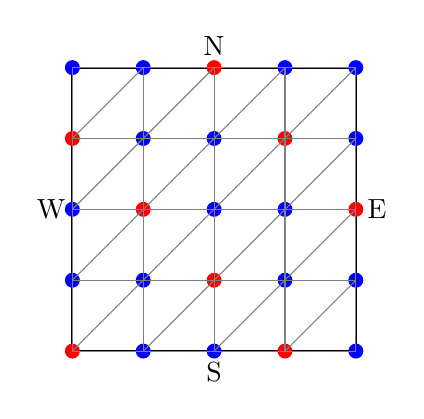
\begin{tikzpicture}[scale=0.9]
        % Square
        \draw[thick] (0,0) rectangle (4,4);
        \node at (2,4.3) {N};
        \node at (2,-0.3) {S};
        \node at (-0.3,2) {W};
        \node at (4.3,2) {E};
        % Grid of vertices
        \foreach \x in {0,1,2,3,4} {
            \foreach \y in {0,1,2,3,4} {
                \pgfmathparse{mod(\x+\y,3)==0 ? 1 : 0}
                \ifnum\pgfmathresult=1
                    \fill[red] (\x,\y) circle (3pt);
                \else
                    \fill[blue] (\x,\y) circle (3pt);
                \fi
            }
        }
        % Triangulation lines (some diagonals)
        \foreach \x in {0,1,2,3} {
            \foreach \y in {0,1,2,3} {
                \draw[gray,thin] (\x,\y) -- (\x+1,\y+1);
            }
        }
        % Horizontal and vertical grid
        \foreach \x in {0,1,2,3,4} {
            \draw[gray,thin] (\x,0) -- (\x,4);
        }
        \foreach \y in {0,1,2,3,4} {
            \draw[gray,thin] (0,\y) -- (4,\y);
        }
    \end{tikzpicture}
    \end{center}

    Suppose there is a coloring for which neither red nor blue connects the two opposite sides. Then, we can construct a continuous map $f \colon I^2 \to I^2$ without any fixed point, which contradicts the Brouwer fixed point theorem.

    We construct such $f$ as follows: For each vertex $v$ of the triangulation, set
    \[
        f(v) = \begin{cases}
            v + (\varepsilon, 0) & \text{if } v \text{ is colored in red and connected to W}, \\
            v - (\varepsilon, 0) & \text{if } v \text{ is colored in red and not connected to W}, \\
            v + (0, \varepsilon) & \text{if } v \text{ is colored in blue and connected to S}, \\
            v - (0, \varepsilon) & \text{if } v \text{ is colored in blue and not connected to S}.
        \end{cases}
    \]
    Extend linearly on each simplex. Then $f$ has no fixed points.
\end{proof}
